\documentclass[letterpaper]{article}
\usepackage{amsmath}
\usepackage{amssymb}
\usepackage{comment}
\usepackage{color}
\usepackage{url}
\usepackage[margin=1in]{geometry}
\usepackage[all]{xy}  % xy-pic
\usepackage{graphicx}  % scalebox

%		custom symbol		%

\newcommand{\Omit}{{\it Refer to the textbook.}}
\newcommand{\Empty}{{\it \color{red} Need a solution.}}
\newcommand{\Error}{{\it \color{red} There is something wrong with the problem.}}
\newcommand{\Star}{$^\star$}
\newcommand{\TT}[1]{\texttt{#1}}
\newcommand{\RM}[1]{\textrm{#1}}
\newcommand{\BF}[1]{\textbf{#1}}
\newcommand{\IT}[1]{\textit{#1}}
\newcommand{\Bra}[1]{\langle {#1} \rangle}
\newcommand{\Leqm}{\leq_{\RM{m}}}
\newcommand{\K}{\RM{K}}
\newcommand{\Poly}{\RM{P}}
\newcommand{\NPoly}{\RM{NP}}
\newcommand{\PSPACE}{\RM{PSPACE}}
\newcommand{\NPSPACE}{\RM{NPSPACE}}
\newcommand{\LeqP}{\leq_{\Poly}}
\newcommand{\BigO}{\mathcal{O}}
\newcommand{\Attr}[1]{{\bf ({#1})}}  % attributed to
\newcommand{\Sol}[1]{\vspace{4pt} \noindent {\bf Solution {#1}. }}

\newcommand{\CFL}{\textsf{CFL}}
\newcommand{\CFG}{\textsf{CFG}}
\newcommand{\DFA}{\textsf{DFA}}
\newcommand{\NFA}{\textsf{NFA}}
\newcommand{\REX}{\textsf{REX}}
\newcommand{\TM}{\textsf{TM}}
\newcommand{\NTM}{\textsf{NTM}}
\newcommand{\PDA}{\textsf{PDA}}
\newcommand{\DPDA}{\textsf{DPDA}}
\newcommand{\LBA}{\textsf{LBA}}

%		initialization		%

\title{Solution to Introduction to the Theory of Computation}
\author{Lwins\_Lights}
\date{}

\begin{document}
	
	\maketitle
	
	\tableofcontents
	
	\section{Chapter 1: Regular Languages}

\begin{itemize}
	
	
	\item[\hard 1.45]
	\begin{comment}
	Let $A/B = \{w \ | \ wx \in A \text{ for some } x \in B \}$. Show that if $A$ is regular and $B$ is any language, then $A/B$ is regular. 
	
	\hint
	\end{comment}
	Let $M = (Q, \Sigma, \delta, q_0, F)$ be a DFA such that $L(M) = A$. Consider $ \{ q \in Q \ | \ \exists x \in B,\ \delta(q, x) \in F \} $.
	
	
	\item[\hard 1.56]
	\begin{comment}
	If $A$ is a set of natural numbers and $k$ is a natural number greater than $1$, let
	\[
		B_k(A) = \{ w \ | \ w \text{ is the representation in base $k$ of some number in $A$} \}.
	\]
	Here, we do not allow leading $\mathtt{0}$s in the representation of a number. For example, $B_2(\{3, 5\}) = \{ \mathtt{11}, \mathtt{101} \}$ and $B_3(\{3, 5\}) = \{ \mathtt{10}, \mathtt{12} \}$. Give an example of a set $A$ for which $B_2(A)$ is regular but $B_3(A)$ is not regular. Prove that your example works.
	
	\hint
	\end{comment}
	Let $A = \{2^n \ | \ n \in \mathbb{N} \}$. You may need to do a bit of algebra or number theory.
	
	
	\item[\hard 1.57] 
	\begin{comment}
	If $A$ is any language, let $A_{\frac{1}{2}-}$ be the set of all first halves of strings in $A$ so that
	\[
		A_{\frac{1}{2}-} = \{ x \ | \ \text{for some $y$, $|x| = |y|$ and $xy \in A$} \}.
	\]
	Show that if $A$ is regular, then so is $A_{\frac{1}{2}-}$.
	
	\hint
	\end{comment}
	Let $M$ be a DFA such that $L(M) = A$. Utilizing $M$, design an NFA which accepts $A_{\frac{1}{2}-}$ by guessing something.
	
	
	\item[\hard 1.58] 
	\begin{comment}
	If $A$ is any language, let $A_{\frac{1}{3}-\frac{1}{3}}$ be the set of all strings in $A$ with their middle thirds removed so that	
	\[
		A_{\frac{1}{3}-\frac{1}{3}} = \{ xz \ | \ \text{for some $y$, $|x| = |y| = |z|$ and $xyz \in A$} \}.
	\]
	Show that if $A$ is regular, then $A_{\frac{1}{3}-\frac{1}{3}}$ is not necessarily regular
	
	\hint
	\end{comment}
	Let $A = \mathtt{a}^* \texttt{\#} \mathtt{b}^*$. 
	
	
	\item[\hard 1.59]
	\begin{comment}
	Let $M = (Q, \Sigma, \delta, q_0, F)$ be a DFA and let $h$ be a state of $M$ called its ``home''. A \bm{synchronizing sequence} for $M$ and $h$ is a string $s \in \Sigma^*$ where $\delta(q, s) = h$ for every $q \in Q$. (Here we have extended $\delta$ to strings, so that $\delta(q, s)$ equals the state where $M$ ends up when $M$ starts at state $q$ and reads input $s$.) Say that $M$ is \bm{synchronizable} if it has a synchronizing sequence for some state $h$. Prove that if $M$ is a $k$-state synchronizable DFA, then it has a synchronizing sequence of length at most $k^3$. Can you improve upon this bound?
	
	\hint
	\end{comment}
	Let $Q'$ stands for some subset of $Q$. Try to design a method that finds a relatively short string $w$ such that $|\delta(Q', w)| < |Q'|$, where $\delta(Q', w) = \{ \delta(q, w) \ | \ q \in Q' \}$.
	
	
	\item[\hard 1.63] 
	\begin{comment}
	\begin{itemize}
		\item[a.]
		Let $A$ be an infinite regular language. Prove that $A$ can be split into two infinite disjoint regular subsets.
		\item[b.]
		Let $B$ and $D$ be two languages. Write $B \Subset D$ if $B \subseteq D$ and $D$ contains infinitely many strings that are not in $B$. Show that if $B$ and $D$ are two regular languages where $B \Subset D$, then we can find a regular language $C$ where $B \Subset C \Subset D$.
	\end{itemize}

	\hint
	\end{comment}
	For part a, use the pumping lemma.


	\item[\hard 1.65]
	\begin{comment}
	Prove that for each $n>0$, a language $B_n$ exists where
	\begin{itemize}
		\item[a.]
		$B_n$ is recognizable by an NFA that has $n$ states, and
		\item[b.]
		if $B_n = A_1 \cup \cdots \cup A_k$ for regular languages $A_i$, then at least one of the $A_i$ requires a DFA with exponentially many states.
	\end{itemize}

	\hint
	\end{comment}
	Consider $B_{n+2} = \Sigma^*\mathtt{1}\mathtt{0}^{n}$.
	
	
	\item[\hard 1.67]
	\begin{comment}
	Let the \bm{rotational closure} of language $A$ be $RC(A) = \{ yx \ | \ xy \in A \}$.
	\begin{itemize}
		\item[a.]
		Show that for any language $A$, we have $RC(A) = RC(RC(A))$.
		\item[b.]
		Show that the class of regular languages is closed under rotational closure.
	\end{itemize}
	\hint
	\end{comment}
	For part b, let $M$ be a DFA such that $L(M) = A$. Utilizing $M$, design an NFA which accepts $RC(A)$ by guessing something.
	
	
	\item[\hard 1.68] 
	\begin{comment}
	In the traditional method for cutting a deck of playing cards, the deck is arbitrarily
	split two parts, which are exchanged before reassembling the deck. In a more
	complex cut, called Scarne’s cut, the deck is broken into three parts and the middle
	part in placed first in the reassembly. We’ll take Scarne’s cut as the inspiration for
	an operation on languages. For a language $A$, let $CUT(A) = \{ yxz \ | \ xyz \in A \}$.
	\begin{itemize}
		\item[a.]
		Exhibit a language $B$ for which $CUT(B) \neq CUT(CUT(B))$.
		\item[b.]
		Show that the class of regular languages is closed under $CUT$.
	\end{itemize}
	\hint
	\end{comment}
	Solve problem 1.67 first.

	
\end{itemize}
	\section{Chapter 2: Context-Free Languages}

\begin{itemize}
	
	
	\item[\hard 2.19]
	\begin{comment}
	Let CFG $G$ be the following grammar.
	\[
		\begin{array}{rcl}
			S & \to & \texttt{a}S\texttt{b} \ | \ \texttt{b}Y \ | \ Y\texttt{a} \\
			Y & \to & \texttt{b}Y \ | \ \texttt{a}Y \ | \ \epsilon
		\end{array}
	\]
	Give a simple description of $L(G)$ in English. Use that description to give a CFG for $\overline{L(G)}$, the complement of $L(G)$.
	
	\hint
	\end{comment}
	$Y \to (\tt{a} \cup \tt{b})^*$ and $S \to \tt{a}^n (\tt{b} Y \cup Y \tt{a}) \tt{b}^n$ where $n \in \mathbb{N}$.
	
	
	\item[\hard 2.21] 
	\begin{comment}
	Let $\Sigma = \{ \tt{a}, \tt{b} \}$. Give a CFG generating the language of strings with twice as many $\tt{a}$'s as $\tt{b}$'s. Prove that your grammar is correct.
	
	\hint
	\end{comment}
	Define $\chi : \Sigma^* \to \mathbb{Z}$ by $\chi(x) = n_{\tt{a}}(x) - 2 n_{\tt{b}}(x)$, where $n_{\tt{a}}(x)$ counts the number of $\tt{a}$s in $x$. Suppose $x = x_1 x_2 \dots x_m$ with $x_i \in \Sigma$. What will happen to $x_l x_{l+1} \cdots x_r$ if $\chi(x_1 x_2 \cdots x_r) = \chi(x_1 x_2 \cdots x_{l-1})$?
	
	
	\item[\hard 2.22] 
	\begin{comment}
	Let $C = \{ x \tt{\#} y \ | \ x,y \in \{\tt{0},\tt{1}\}^* \text{ and } x \neq y \}$. Show that $C$ is a context-free language.
	
	\hint
	\end{comment}
	$C = \{ x \tt{\#} y \ | \ |x| \neq |y| \} \cup \bigcup_{i \in \mathbb{Z}^+} \{ x \tt{\#} y \ | \ |x| = |y| \text{ and } x_i \neq y_i \}$, where $x_i$ is denoted as the $i$-th character of $x$.
	
	
	\item[\hard 2.23]
	\begin{comment}
	Let $D = \{ xy \ | \ x,y \in \{\tt{0},\tt{1}\}^* \text{ and } |x|=|y| \text{ but } x \neq y \}$. Show that $D$ is a context-free language.
	
	\hint
	\end{comment}
	Solve problem 2.22 first.
	
	\item[\hard 2.24]
	\begin{comment}
	Let $E = \{ \tt{a}^i \tt{b}^j \ | \ i \neq j \text{ and } 2i \neq j \}$. Show that $E$ is a context-free language.
	
	\hint
	\end{comment}
	$E = \{ \tt{a}^i \tt{b}^j \ | \ j < i \} \cup \{ \tt{a}^i \tt{b}^j \ | \ i < j < 2i \} \cup \{ \tt{a}^i \tt{b}^j \ | \ j > 2i \} $.
	
	
	\item[\hard 2.27]
	\begin{comment}
	\newcommand{\abrsc}[1]{\abr{\sc{#1}}}
	Let $G = (V, \Sigma, R, \abr{\sc{stmt}})$ be the following grammar.
	\[
		\begin{array}{rcl}
			\abrsc{stmt} & \to & \abrsc{assign} \ | \ \abrsc{if-then} \ | \ \abrsc{if-then-else} \\
			\abrsc{if-then} & \to & \tt{if condition then } \abrsc{stmt} \\
			\abrsc{if-then-else} & \to & \tt{if condition then } \abrsc{stmt} \tt{ else } \abrsc{stmt} \\
			\abrsc{assign} & \to & \tt{a:=1}
		\end{array}
	\]
	$G$ is a natural-looking grammar for a fragment of a programming language, but $G$ is ambiguous.
	\begin{itemize}
		\item[a.]
		Show that $G$ is ambiguous.
		\item[b.]
		Give a new unambiguous grammar for the same language.
	\end{itemize}

	\hint
	\end{comment}
	For part b, try to let every $\tt{else}$ correspond to the nearest $\tt{if}$, like what C/C++ grammar specifies.
	
	
	\item[\hard 2.28]
	Solve problem 2.21 first.
	
	
	\item[\hard 2.29]
	Use the pumping lemma.
	
	
	\item[\hard 2.33]
	Use the pumping lemma on $\tt{a}^{(p+1)^2} \tt{b}^{p+1}$.
	
	
	\item[\hard 2.37]
	$R$'s appearing twice gives us the pumping lemma for CFL. What if it appears thrice?
	
	
	\item[\hard 2.40]
	Use the pumping lemma.
	
	
\end{itemize}
	\section{The Church--Turing Thesis}

	\section{Decidability}

\begin{itemize}
	
	%		4.10		%
	\item[4.10]
	\Omit
	
	%		4.11		%
	\item[4.11]
	By the pumping lemma, $L(M)$ is an infinite language $\iff$ $L(M)$ includes a string of at least length $p$. Since $R = \Sigma^p \Sigma^*$ is a regular language, it is easy to design a \PDA \ $P$ recognizing $L(M) \cap R$. Then use $E_{\PDA}$'s decider to decide whether $L(M) \cap R = \varnothing$.
	
	%		4.12		%
	\item[4.12]
	\Omit
	
	%		4.13		%
	\item[4.13]
	$L(R) \subseteq L(S) \iff L(R) \cup L(S) = L(S)$, which can be decided by $EQ_{\DFA}$'s decider.
	
	%		4.14		%
	\item[4.14]
	\Omit
	
	%		4.15		%
	\item[\Star 4.15]
	By the pumping lemma, $\TT{1}^k \in L(G) \implies \TT{1}^{k+p!} \in L(G)$ for every $k \geq p$. Therefore $\TT{1}^* \subseteq L(G) \iff \{ \TT{1}^k \ | \ k \leq p+p! \} \subseteq L(G)$, which can be easily checked by a \TM \ in finite time.
	
	%		4.16		%
	\item[4.16]
	Since $A = \{ \Bra{R} \ | \ \text{$R$ is a regular expression, } R \cap \Sigma^* \TT{111} \Sigma^* \neq \varnothing \}$, we only need an $E_{\DFA}$'s decider.
	
	%		4.17		%
	\item[4.17]
	Suppose we have two \DFA s $D_1$ and $D_2$. Let $D$ be a \DFA \ recognizing $L(D_1) \oplus L(D_2)$, where $\oplus$ means symmetric difference. By the pumping lemma, $L(D) \cap (\Sigma \cup \epsilon)^p = \varnothing \implies L(D) = \varnothing$, thus $p$ can be the required length.
	
	%		4.18		%
	\item[\Star 4.18] 
	\begin{itemize}
		\item[$\Leftarrow$:] It is enough to design a \TM , which recognizes $C$ by checking whether $\Bra{x,y} \in D$ for all possible $y$ one by one.
		\item[$\Rightarrow$:] Suppose \TM \ $M$ recognizes $C$. Let $D = \{ \Bra{x,y} \ | \ x \in C$  and $y$ is the computation history of $M$ on input $x \}$, which is obviously decidable.
	\end{itemize}

	%		4.19		%
	\item[\Star 4.19]
	Let $C$ be a recognizable but undecidable language, e.g., $A_{\TM}$. Construct $D$ provided by Problem 4.18. Letting homomorphism $f$ satisfy $f(\Bra{x,y}) = x$ for every $x,y$ we obtain $f(D) = C$.
	
	%		4.20		%
	\item[4.20]
	Let $M$ be a \TM \ which runs both $\overline{A}$'s recognizer and $\overline{B}$'s recognizer on its own input. $M$ accepts when $\overline{B}$'s recognizer accepts and rejects when $\overline{A}$'s recognizer accepts. Clearly $C = L(M)$ separates $A$ and $B$.
	
	%		4.21		%
	\item[4.21]
	$M$ is a \DFA \ that accepts $w^\mathcal{R}$ whenever it accepts $w$ $\iff$ $L(M) = L(M)^\mathcal{R}$, which can be decided by $EQ_{\DFA}$'s decider.
	
	%		4.22		%
	\item[4.22]
	In order to determine whether $L(R)$ is prefix-free, it suffices to check whether the \DFA \ recognizing $L(R)$ has the property that from a reachable accept state we could arrive an accept state again by several transitions.
	
	%		4.23		%
	\item[\Star 4.23]
	\Omit
	
	%		4.24		%
	\item[4.24]
	A \PDA \ $P = (Q, \Sigma, \Gamma, \delta, q_0, F)$ has an useless state $q \in Q$ if and only if \PDA \ $P' = (Q, \Sigma, \Gamma, \delta, q_0, \{q\})$ recognizes $\varnothing$. Therefore we can use $E_{\PDA}$'s decider to solve it.
	
	%		4.25		%
	\item[\Star 4.25]
	\Omit
	
	%		4.26		%
	\item[\Star 4.26] 
	$M$ is a \DFA \ that accepts some palindrome $\iff$ \CFL \ $\{ w \ | \ w = w^{\mathcal{R}} \} \cap L(M)$ is not empty, which can be decided by $E_{\PDA}$'s decider.
	
	%		4.27		%
	\item[\Star 4.27] 
	Refer to the solution to Problem 4.26.
	
	%		4.28		%
	\item[4.28]
	$x$ is a substring of some $y \in L(G)$ $\iff$ $L(G) \cap \Sigma^* x \Sigma^* \neq \varnothing$, which can be decided by $E_{\PDA}$'s decider.
	
	%		4.29		%
	\item[4.29]
	By the pumping lemma, $L(G)$ is an infinite language $\iff$ $L(G)$ includes a string of at least length $p$. So we can first use $\IT{INFINITE}_{\PDA}$ from Problem 4.11 to check whether $|L(G)| = \infty$, and then check whether $x \in L(G)$ for all $x$ of less-than-$p$ length, one by one.
	
	%		4.30		%
	\item[4.30]
	Let $E$ be $A$'s enumerator which generates $\Bra{M_1}, \Bra{M_2}, \dots$ in order. Construct $D = \{ \Bra{n} \ | \ \Bra{n} \notin L(M_n) \}$.
	
	%		4.31		%
	\item[4.31]
	First, recursively determine whether $V \overset{*}{\Rightarrow} w$ with some $w \in \Sigma^*$, for all variables $V$. Then, recursively determine whether $V \overset{*}{\Rightarrow} xAy$ with some $x, y \in \Sigma^*$, for all variables $V$.
	
	%		4.32		%
	\item[4.32]
	Construct \DPDA\ $P'_{(q,x)}$ by modifying $P$, such that $L(P'_{(q,x)}) = \varnothing$ if and only if $(q, x)$ is a looping situation for $P$. Then we only need $E_{\PDA}$.
	
\end{itemize}
	\section{Reducibility}

\begin{itemize}
	
	%		5.9			%
	\item[5.9]
	Reduce to $A_{\TM}$. To determine whether \TM\ $M$ accepts $w$, construct \TM\ $N$ which always accepts $\TT{01}$ but accepts $\TT{10}$ if and only if $M$ accepts $w$.
	
	%		5.10		%
	\item[5.10]
	\Omit
	
	%		5.11		%
	\item[5.11]
	\Omit
	
	%		5.12		%
	\item[5.12]
	Reduce to $E_{\TM}$. To determine whether \TM\ $M$ accepts nothing, construct \TM\ $N$ which simulates $M$ on $N$'s own input $w$ but never writes a blank symbol over a nonblank symbol unless when $M$ accepts.
	
	%		5.13		%
	\item[5.13]
	Reduce to $E_{\TM}$. To determine whether \TM\ $M$ accepts nothing, construct \TM\ $N$ which simulates $M$ on $N$'s own input $w$ and obviously has no useless state except the one $q_{\RM{accept}}$.
	
	%		5.14		%
	\item[5.14]
	\Empty
	
	%		5.15		%
	\item[5.15]
	Let $M'$ be $M$ after modifying all its transitions $\delta(q_i,a) = (q_{\RM{accept}},b,X)$ to $\delta(q_i,a) = (q_{\RM{reject}},b,X)$, and then modifying all $\delta(q_i,a) = (q_j,b,\RM{L})$ to $\delta(q_i,a) = (q_{\RM{accept}},b,\RM{R})$. The problem is now reduced to checking whether $M'$, as a \emph{\TM\ with stay put instead of left} described in problem 3.13, accepts $w$. It is easy since $L(M')$ is regular by the solution to problem 3.13.
	
	%		5.16		%
	\item[5.16]
	Suppose for the sake of contradiction that $BB$ is computable. Then obviously there exists a \TM\ $M$ having $k$ states, which writes $BB(n) + 1$ \TT{1}s on the tape, when given input $\Bra{n}$. Further, using $M$ we can construct a series of \TM s $M_n$ having exactly $k+n/2$ states, which writes $BB(n) + 1$ \TT{1}s on the tape when started with a blank tape. However, then $M_{2k}$, as a $2k$-state \TM , would write $BB(2k) + 1$ \TT{1}s. Absurd.
	
	%		5.17		%
	\item[5.17]
	\Empty
	
	%		5.18		%
	\item[5.18]
	\Empty
	
	%		5.19		%
	\item[5.19]
	\Empty
	
	%		5.20		%
	\item[5.20]
	\Empty
	
	%		5.21		%
	\item[5.21]
	The hint in the textbook is sufficient.
	
	%		5.22		%
	\item[5.22]
	\begin{itemize}
		\item[$\Leftarrow$:] Trivial.
		\item[$\Rightarrow$:] Let $f(x) = \Bra{M, x}$, where \TM\ $M$ is $A$'s recognizer. 
	\end{itemize}

	%		5.23		%
	\item[5.23]
	\begin{itemize}
		\item[$\Leftarrow$:] Trivial, since $\TT{0}^*\TT{1}^*$ is surely decidable.
		\item[$\Rightarrow$:] Suppose there is an $A$'s decider, then $f$ defined as follows is computable.
		\[
			f(x) = 
			\left\{
				\begin{array}{ll}
					\TT{01}, & x \in A \\
					\TT{10}, & x \notin A
				\end{array}
			\right.
		\]
	\end{itemize}

	%		5.24		%
	\item[5.24]
	\Empty
	
	%		5.25		%
	\item[5.25]
	$\overline{E_{\TM}} \Leqm A_{\TM}$ by problem 5.22 and it is well known that $A_{\TM} \Leqm E_{\TM}$. By the way, it is not difficult to construct an undecidable language $B$ such that $B =_{\RM{m}} \overline{B}$.
	
\end{itemize}
	\section{Advanced Topics in Computability Theory}

\begin{itemize}
	
	%		6.6			%
	\item[6.6]
	Let $M = P_{\Bra{N}}$ and $N$ print $q(\Bra{N}) = \Bra{M}$.
	
	%		6.7			%
	\item[6.7]
	A \TM\ that always loops.
	
	%		6.8			%
	\item[\Star 6.8]
	Suppose for the sake of contradiction that $f$ is a reduction from $EQ_{\TM}$ to $\overline{EQ_{\TM}}$. It is easy to generalize the fixed-point version of the recursion theorem to find $f(\Bra{M, N}) = \Bra{M', N'}$ such that $M, N$ simulate $M', N'$ respectively. Then $\Bra{M, N} \in EQ_{\TM} \iff \Bra{M', N'} \in \overline{EQ_{\TM}} \iff \Bra{M, N} \in \overline{EQ_{\TM}}$. Absurd.
	
	%		6.9			%
	\item[6.9]
	\Omit
	
	%		6.10		%
	\item[6.10]
	\Omit
	
	%		6.11		%
	\item[\Star 6.11]
	$(\mathbb{R}, =, <)$.
	
	%		6.12		%
	\item[6.12]
	\Omit
	
	%		6.13		%
	\item[6.13]
	Since $\mathbb{Z}_m$ is finite, any sentence in the language of $\mathcal{F}_m$ can be decided by brute-force checking.
	
	%		6.14		%
	\item[6.14]
	Let $J = \TT{0}A \cup \TT{1}B$.
	
	%		6.15		%
	\item[6.15]
	Let $B = A_{\TM^A} = \{ \Bra{M^{A}, w} \ | \ \text{$M^A$ accepts $w$} \}$. Then apply any classical method used in proving undecidablity of $A_{\TM}$.
	
	%		6.16		%
	\item[\Star 6.16]
	\Attr{Kleene--Post} For convenience let any language $L$ be a subset of $\mathbb{N}$ instead of $\Sigma^*$. Denote $\{0, 1, \dots, m\}$ by $[m]$. Define 
	$$
		\mathcal{L}_m(A) = \{ L \subseteq \mathbb{N} \ | \ L \cap [m] = A\} \quad (A \subseteq [m])
	$$
	Let $M_0, M_1, M_2, \dots$ be all possible oracle \TM s. We will give two series of families of languages $\mathcal{A}_0 \supseteq \mathcal{A}_1 \supseteq \mathcal{A}_2 \supseteq \cdots$ and $\mathcal{B}_0 \supseteq \mathcal{B}_1 \supseteq \mathcal{B}_2 \supseteq \cdots$ such that
	$$
		\forall A \in \mathcal{A}_n, B \in \mathcal{B}_n,\ M_n^A \text{ is not $B$'s decider} \text{ and } M_n^B \text{ is not $A$'s decider}.
	$$
	Then taking arbitrary $A \in \mathcal{A} = \bigcap_{n \in \mathbb{N}} \mathcal{A}_n$ and $B \in \mathcal{B} = \bigcap_{n \in \mathbb{N}} \mathcal{B}_n$ we have $A \nleq_{\RM{T}} B$ and $B \nleq_{\RM{T}} A$. We build them by induction. Given $\mathcal{A}_{n-1} = \mathcal{L}_m(X)$ and $\mathcal{B}_{n-1} = \mathcal{L}_m(Y)$, we first find $\mathcal{A}'_n \subseteq \mathcal{A}_{n-1}$ and $\mathcal{B}'_n \subseteq \mathcal{B}_{n-1}$ such that $\forall A \in \mathcal{A}'_n, B \in \mathcal{B}'_n,\ M_n^A \text{ is not $B$'s decider}$.
	\begin{itemize}
		\item If there is no $A \in \mathcal{A}_{n-1}$ such that $M_n^A$ is a decider, let $\mathcal{A}'_n = \mathcal{A}_{n-1}$ and $\mathcal{B}'_n = \mathcal{B}_{n-1}$.
		\item Suppose $M_n^A$ is a decider with some $A \in \mathcal{A}_{n-1}$, then there exists an $m'>m$ such that 
		$$
			\forall A' \in \mathcal{L}_{m'}(A \cap [m']),\ m+1 \in L(M_n^A) \iff m+1 \in L(M_n^{A'}).
		$$
		Then, let $\mathcal{A}'_n = \mathcal{L}_{m'}(A \cap [m'])$, $\mathcal{B}'_n = \mathcal{L}_{m'}(Y)$ or $\mathcal{L}_{m'}(Y \cup \{m+1\})$, depending on whether $m+1 \in L(M_n^A)$.
	\end{itemize}
	The same method can be also used to find $\mathcal{A}_n \subseteq \mathcal{A}'_{n}$ and $\mathcal{B}_n \subseteq \mathcal{B}'_{n}$ such that $\forall A \in \mathcal{A}_n, B \in \mathcal{B}_n,\ M_n^B $ is not $A$'s decider.
	
	%		6.17		%
	\item[\Star 6.17]
	Let 
	\begin{align*}
		A = \{ \Bra{M, w} \ | \ \text{\TM\ $M$ on input $w$ halts with \TT{0} on its tape} \} \\
		B = \{ \Bra{M, w} \ | \ \text{\TM\ $M$ on input $w$ halts with \TT{1} on its tape} \}
	\end{align*}
	If there is a $C$'s decider $N$, we can construct \TM\ $M$ which on input $w$ first run $N$ on $\Bra{M, w}$ to know that $M$ would not halt with $x \in \{ \TT{0}, \TT{1} \}$ on $M$'s tape, and then violates it.
	
	%		6.18		%
	\item[6.18]
	Suppose $L(M) \neq L(N)$, we can enumerate $x$ to find one such that $\Bra{M, x} \in A_{\TM} \oplus \Bra{N, x} \in A_{\TM}$ holds, where $\oplus$ means exclusive or.
	
	%		6.19		%
	\item[6.19]
	$ |\{ L(M^A) \ | \ \text{$M^A$ is an oracle \TM} \}| \leq |\{ M^A \ | \ \text{$M^A$ is an oracle \TM} \}| \leq \aleph_0 < 2^{\aleph_0} = |\{ L \ | \ \text{$L$ is a language} \}|$.
	
	%		6.20		%
	\item[6.20]
	Let $M$ be $PCP$'s recognizer. Then check whether $\Bra{M, \Bra{P}} \in A_{\TM}$ to know if instance $P$ has a match.
	
	%		6.21		%
	\item[6.21]
	Since $\K(x) \leq |x| + c$, we can check all possible minimal description $\Bra{M, w}$ to see if $M$ on input $w$ halts with $x$ on its tape by simulating $M$, where ``possible'' means that $|\Bra{M, w}| < |x| + c$ and $\Bra{M, w} \in A_{\TM}$.
	
	%		6.22		%
	\item[6.22]
	Trivial.
	
	%		6.23		%
	\item[6.23]
	Reduce from Problem 6.24.
	
	%		6.24		%
	\item[6.24]
	Reduce from Problem 6.25.
	
	%		6.25		%
	\item[6.25]
	If not, there is an enumerator $E$ which would print infinite many incompressible strings one by one: $s_1, s_2, \dots$ By using $E$ we can construct \TM\ $M$, which prints an incompressible string $s_i$, such that $|s_i| > |\Bra{M, \TT{0}}|$, on its tape. Then we have $\K(s_i) \leq |\Bra{M, \TT{0}}| < |s_i|$. Absurd.
	
	%		6.26		%
	\item[\Star 6.26] 
	\Sol{1}
	Suppose for the sake of contradiction that $\K(xy) \leq \K(x) + \K(y) + c$ always holds. Define
	$$
		f_n = \sum_{|x|=n} {2^{-\K(x)}}.
	$$
	Then $\K(xy) \leq \K(x) + \K(y) + c \implies f_{n+m} \geq 2^{-c} f_n f_m \implies f_{k n} \geq (2^{-c} f_n)^{k}$. On the other hand, Corollary 6.30 implies $f_n \leq n + 1$. Therefore, 
	$$
		f_n \leq 2^c \sqrt[k]{f_{k n}} \leq 2^c \sqrt[k]{kn + 1}.
	$$
	Letting $k \to +\infty$ we obtain that $f_n \leq 2^c$ for all $n$. However, there is a \TM\ $M$ which on input $\Bra{p, q}$ ($p, q \in \mathbb{N}$ and $q < 2^{2^p}$) halts with $r(p,q)$, a $2^p$-bits binary representation of $q$, on its tape. So $\K(r(p,q)) \leq 2 \log_2 p + \log_2 q + d$ with some constant $d$. Then, if $n = 2^p$ for some large $p$,
	$$
		f_{n} = \sum_{|x|=n} {2^{-\K(x)}} \geq \sum_{q < 2^n} {2^{-\K(r(p,q))}} \geq 2^{-2 \log_2 p - d} \sum_{q < 2^n} \frac{1}{q} \geq \frac{n}{2^d (\log_2 n)^2},
	$$
	which apparently contradicts with $f_n \leq 2^c$.
	
	\Sol{2}
	$ \forall c $, the following process of choosing $ x $ and $ y $ constructs the inequality directly.
	
	First, select an incompressible string $ w $ with length $ n $. Denote its prefix string of length $ \frac{1}{2} \log n $ as $ u $. Let number $ p $ equal the value of $ 1u $ when perceived as a  binary number.
	
	Then, divide $ w $ into two substrings $ w=xy $, where $ \left| x \right| = \frac{1}{2} \log n + p $ and $ \left| y \right| = n - \left| x \right| $ (since $ p < 2^{\frac{1}{2} \log n + 1} = 2 \sqrt{n}$, $ \left| y \right| > 0 $ is a valid string as long as $ n $ is large enough).
	
	We observe that since $ w $ is incompressible, $ K(xy) \ge n $. Also, $ K(y) \le \left| y \right| + c_1 $ for some constant $ c_1 $ independent of $ n $.
	
	We claim that $ K(x) \le p + c_2 $ for some constant $ c_2 $ independent of $ n $. In fact, the following Turing machine $ M $ generates $ x $ when the input string is the tail string of $ x $ with length $ p $:
	
	M="With input string $ z $:
	
	~~~~~~Calculate $ q = \left| z \right| $ and write $ q $ in binary representation on the tape;
	
	~~~~~~Remove the leading character 1 of $ q $, append $ q $ with $ z $, and output them together."
	
	Now, with all the above claims, we get $ K(xy) - \left( K(x) + K(y) + c \right) \ge \frac{1}{2} \log n - \left( c_1 + c_2 + c \right) > 0 $ as long as $ n $ is large enough.
	
	%		6.27		%
	\item[6.27]
	Show that $\overline{\IT{HALT}_{\TM}} \Leqm S, \overline{S}$.
	
	%		6.28		%
	\item[6.28]
	\begin{enumerate}
		\item[a.] $x = 0 \iff \forall y,\ x+y=y$
		\item[b.] $x = 1 \iff \forall y,\ y=0 \wedge x+y=1$ 
		\item[c.] $x = y \iff \forall z,\ z=0 \wedge x+z=y$
		\item[d.] $x < y \iff \exists z,\ \neg(z = 0) \wedge x + z = y$
	\end{enumerate}
	
\end{itemize}

	\section{Time Complexity}

\begin{itemize}
	
	%		7.13		%
	\item[7.13]
	$a^b = (a^{\lfloor b/2 \rfloor})^2 \cdot a^{b \bmod 2}$, where $a, b \in \mathbb{N}$.
	
	%		7.14		%
	\item[7.14]
	$q^t = (q^{\lfloor t/2 \rfloor})^2 \cdot q^{t \bmod 2}$, where $q \in S_k$ and $t \in \mathbb{N}$.
	
	%		7.15		%
	\item[7.15] 
	The hint in the textbook is sufficient.
	
	%		7.16		%
	\item[7.16]
	\Omit
	
	%		7.17		%
	\item[7.17]
	Use dynamic programming. Denote $dp[i][j] = \boldsymbol{1}\{ \Bra{\{x_1, \dots, x_i\}, j} \in \IT{SUBSET-SUM} \}$, where $\alpha \implies \boldsymbol{1}\{\alpha\} = 1$ and $\neg \alpha \implies \boldsymbol{1}\{\alpha\} = 0$.
	
	%		7.18		%
	\item[7.18]
	First $A \in \Poly = \NPoly$. Then since there exist $x \in A$ and $y \notin A$, for an arbitrary language $B \in \NPoly = \Poly$, $f$ defined as follows is polynomial time computable.
	$$
		f(w) = 
		\left\{
			\begin{array}{ll}
				x, & w \in B \\
				y, & w \notin B
			\end{array}
		\right.
	$$
	
	%		7.19		%
	\item[\Star 7.19]
	Let the certificate of $q \in \mathbb{P}$ consist of
	\begin{itemize}
		\item $g \in \mathbb{Z}_m^*$ such that $g^{m-1}=1$ and $g^{(m-1)/q} \neq 1$ for all prime $q \ | \ m-1$,
		\item the standard factorization of $m-1 = \prod q_i^{r_i}$,
		\item certificates of $q_i \in \mathbb{P}$.
	\end{itemize} 

	%		7.20		%
	\item[7.20]
	It follows from the result of Problem 7.18.
	
	%		7.21		%
	\item[7.21]
	\begin{itemize}
		\item[a.] Modify the proof of $\textit{PATH} \in \Poly$.
		\item[b.] It is in $\NPoly$ evidently. For the other side, reduce from $\IT{UHAMPATH}$ by setting $k$ to the amount of nodes in $G$ minus $1$.
	\end{itemize}

	%		7.22		%
	\item[7.22]
	It is in $\NPoly$ evidently. For the other side, reduce from $\IT{SAT}$. In order to determine whether $\Bra{\phi} \in \IT{SAT}$, construct $\phi' = \phi \,\wedge\,(z \vee \overline{z})$.
	
	%		7.23		%
	\item[7.23]
	\Omit
	
	%               7.25            %
	\item[7.25]
	If there is no unitary negated clause in $ \phi $, then $ \phi $ is satisfiable since we can just assign value 1 to all variables. However, if $ \phi $ contains some clauses in the form $ (\overline{x_i}) $, then this implies that the only possible way to make $ \phi $ true is to let those $ x_i $ equal 0. So $ \phi $ can be reduced to some shorter formula repeatedly.
	
	%		7.36		%
	\item[\Star 7.36] 
	It is in $\NPoly$ evidently. For the other side, reduce from $\IT{3SAT}$. If there is no limitation on $\Sigma$, let the following \DFA\ correspond to an assignment to variables $x_1, x_2, \dots, x_n$ in 3cnf-formula $\phi$. You may need some extra states and transitions.
	$$
		\xymatrix@ur@R=2pc@C=2pc{
			*+[o][F-]{\RM{S}} \ar@(l,l)[]^{} \ar@/^/[r]^{\{ \TT{x}_i | x_i = 1 \}} \ar@/_/[d]_{\{ \TT{x}_i | x_i = 0 \}} &
			*+[o][F-]{T} \ar^{\TT{t}}[d] \ar^{\TT{f}}[l] \\
			*+[o][F-]{F} \ar_{\TT{f}}[r] \ar_{\TT{t}}[u] & 
			*+[o][F-]{A} \ar@(ur,rd)[]^{\Sigma}
		}
	$$
	Once you solved the problem without regard to the limitation on $\Sigma$, based on your solution, consider how to build a reduction where $\Sigma = \{ \TT{0}, \TT{1} \}$.
	
	%		7.37		%
	\item[7.37]
	Using the computation history as certificate we easily obtain $U \in \NPoly$. And it is easy to show that $\IT{3SAT} \LeqP U$, by designing an \NTM\ $M$, which accepts $\Bra{\phi}$ in polynomial time on at least one branch if and only if $\Bra{\phi} \in \IT{3SAT}$.
	
	%		7.38		%
	\item[\Star 7.38]
	Let $\phi(x/t)$ denote the Boolean formula $\phi$ after replacing every existance of $x$ in $\phi$ with $t$. Suppose there are $n$ variables $x_1, \dots, x_n$ in $\phi$. $\Bra{\phi} \in \IT{SAT} \implies \Bra{\phi(x_1/0)} \in \IT{SAT} \text{ or } \Bra{\phi(x_1/1)} \in \IT{SAT}$, so we can directly assign $0$ or $1$ to $x_1$. Recursively assigning $x_2, \dots, x_n$ in this way we have done.
	
	%		7.39		%
	\item[\Star 7.39]
	Construct language $L = \{ \Bra{n, x, y} \ | \ \text{$n$ has a nontrivial factor in interval $[x, y]$} \}$, which is apparently in $\NPoly = \Poly$. Then refer to the solution to Problem 7.38.
	
	%		7.40		%
	\item[\Star 7.40] 
	\Omit
	
	%		7.41		%
	\item[7.41]
	Trivial.
	
	%		7.42		%
	\item[\Star 7.42]
	For b), note that the complement graph of $G$ induces an equivalence relation $\sim$ on $Q$ ($[q]$ is exactly the equivalence class under $\sim$ including $q$), which has much to do with $\equiv_{L(M)}$ defined in Problem 1.51.
	
	%		7.43		%
	\item[7.43]
	Here is a sample for $\phi = (x_1 \vee \overline{x_2} \vee x_3) \wedge (x_2 \vee \overline{x_3})$.
	$$
	\xymatrix@R=2pc@C=2pc{
		*+<1pc>[o][F-]{S} \ar@(l,l)[]^{} \ar[r]^{\epsilon} \ar[rd]_{\epsilon} & 
		*+[o][F-]{A_0} \ar[r]^{\TT{0}} & 
		*+[o][F-]{A_1} \ar[r]^{\TT{1}} & 
		*+[o][F-]{A_2} \ar[r]^{\TT{0}} &
		*+[o][F-]{A_3} \ar[rd]^{\epsilon} \\ & 
		*+[o][F-]{B_0} \ar[r]^{\TT{0} \cup \TT{1}} & 
		*+[o][F-]{B_1} \ar[r]^{\TT{0}} & 
		*+[o][F-]{B_2} \ar[r]^{\TT{1}} &
		*+[o][F-]{B_3} \ar[r]^{\epsilon} &
		*+<1pc>[o][F=]{T}
		% *+[o][F-]{\RM{S}} \ar@/^/[r]^{\{ \TT{x}_i | x_i = 1 \}} \ar@/_/[d]_{\{ \TT{x}_i | x_i = 0 \}} &
		% *+[o][F-]{T} \ar^{\TT{t}}[d] \ar^{\TT{f}}[l] \\
		% *+[o][F-]{F} \ar_{\TT{f}}[r] \ar_{\TT{t}}[u] & 
		% *+[o][F-]{A} \ar@(ur,rd)[]^{\Sigma}
	}
	$$
	And $\Bra{\phi} \notin \IT{SAT} \iff $ the equivalent minimal \NFA\ is a trivial one.
	
	%		7.44		%
	\item[\Star 7.44]
	It is a classical problem. See \url{https://en.wikipedia.org/wiki/2-satisfiability} or refer to Problem 7.51.
	
	%		7.45		%
	\item[7.45]
	Trivial.
	
	%		7.46		%
	\item[7.46]
	Since $P$ is closed under complement, we only need to show that $\overline{\IT{MIN-FORMULA}} \in \NPoly = \Poly$. It is easy to do because $\IT{SAT} \in \NPoly = \Poly$, and then the certicifate for $\Bra{\phi} \in \overline{\IT{MIN-FORMULA}}$ can be $\Bra{\phi'}$ such that $|\phi'| < |\phi|$ and they are equivalent.
	
	%		7.47		%
	\item[7.47]
	$Z = \{ \Bra{G_1, k_1, G_2, k_2} \ | \ \Bra{G_1, k_1} \in \IT{CLIQUE} \} - \{ \Bra{G_1, k_1, G_2, k_2} \ | \ \Bra{G_2, k_2} \in \IT{CLIQUE} \} $.
	
	%		7.48		%
	\item[\Star 7.48]
	Obviously $\IT{MAX-CLIQUE} \in \RM{DP}$. Suppose there is a graph $G = (V, E)$ with $V = \{v_1, v_2, \dots, v_n \}$. Denote $[n] = \{1, 2, \dots, n\}$. Let $G_+ = (V_+, E_+)$, where
	$$
		\left\{
			\begin{array}{l}
				\displaystyle
				V_+ = \{ (i, v_j) \ | \ i \in [n + 1],\ v_j \in V \} \cup \{ (i, \alpha) \ | \ i \in [n+1] - [k] \} \\
				E_+ = \{ \{ (i, u), (j, v) \} \ | \ i \neq j,\ \{u, v\} \in E \} \cup \{ \{ (i, \alpha), (j, v) \} \ | \ i \neq j,\ v \in V \cup \{\alpha\} \}
			\end{array}
		\right.
	$$
	Then $\Bra{G, k} \in \IT{CLIQUE} \iff \Bra{G_+, n+1} \in \IT{MAX-CLIQUE}$. Let $G_-$ consist of $G_+$ and a $n$-clique (i.e., complete graph $K_n$). Then $\Bra{G, k} \notin \IT{CLIQUE} \iff \Bra{G_-, n} \in \IT{MAX-CLIQUE}$. Try to build a reduction by taking advantage of $G_+$ and $G_-$.
	% And we show that $Z \leq_{\RM{T}}^{\Poly} \IT{MAX-CLIQUE}$, where $Z$ is defined in Problem 7.47. To determine whether $\Bra{G_1, k_1, G_2, k_2} \in Z$, we first use the oracle for $\IT{MAX-CLIQUE}$ repeatedly to find the size of largest clique in $G_1$ and $G_2$, denoted as $l_1$ and $l_2$ respectively. Then $\Bra{G_1, k_1, G_2, k_2} \in Z \iff k_1 \leq l_1,\ k_2 > l_2$.
	
	%		7.49		%
	\item[\Star 7.49]
	\Empty
	
	%		7.50		%
	\item[\Star 7.50] 
	$\overline{EQ_{\textsf{SF-REX}}} = \{ \Bra{R, S} \ | \ \exists c,\ c \in L(R) \oplus c \in L(S) \}$. Determining whether $c \in L(R)$ can be achieved in (deterministic) polynomial time by constructing a corresponding \NFA . Note that any $c \in L(R)$ for a star-free \REX\ satisfies $|c| \leq \RM{Poly}(|R|)$.
	
	%		7.51		%
	\item[\Star 7.51] 
	Trivial.
	
	%		7.52		%
	\item[\Star 7.52]
	\Empty
	
	%		7.53		%
	\item[\Star 7.53]
	\Empty
	
	%		7.54		%
	\item[7.54]
	\Empty
	
\end{itemize}

	\section{Space Complexity}

\begin{itemize}
	
	%		8.8			%
	\item[8.8]
	Refer to Example 8.4.
	
	%		8.9			%
	\item[8.9]
	Build an \NTM\ which nondeterministically guesses a ladder $s, s_2, \dots, s_k$ and verifies whether $s_k = t$, where $k$ is obviously bounded in $2^{\mathcal{O}(|s|)}$. Then $\IT{LADDER}_{\DFA} \in \NPSPACE = \PSPACE$ follows.
	
	%		8.10		%
	\item[8.10]
	It can be reduced to $\IT{FORMULA-GAME}$ directly.
	
	%		8.11		%
	\item[8.11]
	If so, $\IT{SAT}$ is \PSPACE -hard, thus it is \PSPACE -complete.
	
	%		8.12		%
	\item[8.12]
	It is because $\phi_{c_1, c_2, 1}$ in the proof of Theorem 8.9 can be written in conjunctive normal form, as we see in the proof of Theorem 7.37 (Cook--Levin theorem).
	
	%		8.13		%
	\item[8.13]
	Reduce from $\IT{TQBF}$. Clearly we can construct a $g(n) = n^{100}+10^{100}$ space \TM\ $M$ deciding $\IT{TQBF}$. Build mapping $f(\Bra{\phi}) = \Bra{M', \Bra{\phi}\TT{\$0}^{g(|\Bra{\phi}|)}}$, where \LBA\ $M'$ does almost the same as $M$ does. On the other side, obviously $A_{\LBA} \in \PSPACE$.
	
	%		8.14		%
	\item[\Star 8.14]
	For any $\Bra{G, c, m, h}$, here is a polynomial time algorithm. Let $C[i][j] = +1$ or $-1$ stand for that we can determine $\Bra{G, i, j, h} \in \IT{HAPPY-CAT}$ or $\Bra{G, i, j, h} \in \IT{HAPPY-MOUSE}$. Similarly let $M[i][j] = +1$ or $-1$ stand for that we can determine $\Bra{G, i, j, h} \in \IT{HAPPY-MOUSE'}$ or $\Bra{G, i, j, h} \in \IT{HAPPY-CAT'}$, where $\IT{HAPPY-CAT'}$ is defined like $\IT{HAPPY-CAT}$, except that Mouse moves first. Now we set $M[i][i] = -1$ and $C[i][h] = -1$ for all $i \in G$. Then, repeatedly assign new value to $M$ and $C$ according to the following rules until we get nothing more from the rules.
	$$
		\left\{
			\begin{array}{ll}
				C[i][j] = -1, & \forall i' \in N(i),\ M[i'][j] = +1 \\
				C[i][j] = +1, & \exists i' \in N(i),\ M[i'][j] = -1 \\
				M[i][j] = -1, & \forall j' \in N(j),\ C[i][j'] = +1 \\
				M[i][j] = +1, & \exists j' \in N(j),\ C[i][j'] = -1
			\end{array}
		\right.
	$$
	where $N(v)$ stands for the collection of all nodes adjacent to $v$ in $G$. After this calculation, we claim that $\Bra{G, c, m, h} \in \IT{HAPPY-CAT} \iff C[c][m] = +1$. The proof of correctness of the algorithm is not evident but also not hard.
	
	%		8.15		%
	\item[8.15]
	\Empty
	
	%		8.16		%
	\item[8.16]
	\Empty
	
	%		8.17		%
	\item[8.17]
	A left-to-right scan with memorizing the amount of non-matched \TT{(}s is enough.
	
	%		8.18		%
	\item[\Star 8.18] 
	Let $h$ be a homomorphism that maps brackets to parentheses, e.g., $h(\TT{([)][]}) = \TT{(())()}$. Denote the substring of $w$ from the $i$-th character to the $j$-th character as $w_{[i,j]}$ and $w_i = w_{[i,i]}$. Then, $w \in B$ if and only if
	\begin{itemize}
		\item $h(w) \in A$, where $A$ is defined in Problem 8.17.
		\item $w_i$ matches $w_j$ whenever $h(w_{[i+1,j-1]}) \in A$, for all $1 \leq i \leq j \leq |w|$.
	\end{itemize}

	%		8.19		%
	\item[\Star 8.19] 
	It is a classical problem. See \url{https://en.wikipedia.org/wiki/Nim}. 
	
	%		8.20		%
	\item[8.20]
	\Empty
	
	%		8.21		%
	\item[8.21]
	\Empty
	
	%		8.22		%
	\item[8.22]
	\Empty
	
	%		8.23		%
	\item[\Star 8.23]
	Suppose $G = (V, E)$ has $n$ nodes named $v_0, v_1, \dots, v_{n-1}$ and define $v_k = v_{k \bmod n}$. Consider the sequence consisting of \emph{directed} edges in $G$, by seeing an undirected edge as two directed ones: $w_0, w_1, w_2, \dots$, where
	$$
		w_{m+1} = (v_j, v_k) \text{, if $w_m = (v_i, v_j)$ and $\{v_j, v_{i+1}\}, \{v_j, v_{i+2}\}, \dots, \{v_j, v_{k-1}\} \notin E$.}
	$$
	$G$ contains no cycle if and only if for every $w_0 = (u, v)$, the first $w_r$ in the sequence such that $w_r = (\cdot, u)$ is $(v, u)$. You may assume $G$ is connected without loss of generality and then use mathematical induction on $n$ to prove this. Note that the sequence $w_0, w_1, w_2, \dots$ would traverse every edges in $G$, i.e., perform depth-first search, if $G$ is a tree.
	
	%		8.24		%
	\item[\Star 8.24]
	\Sol{1}
		Let $N_i^{(n)}$ be an \NFA\ given as follows, with $\Sigma = \{\TT{x}_1, \dots, \TT{x}_n\}$.
		$$
			\xymatrix@R=3pc@C=2pc{
				& *+<1pc>[o][F=]{D} \ar@(lu,ru)[]^{\Sigma} & \\
				*+<1pc>[o][F=]{0} \ar@(l,l)[]^{} \ar@(ld,rd)[]_{\{ \TT{x}_j | j < i \}} \ar@/_/[rr]_{\TT{x}_i} \ar[ru]^{\{ \TT{x}_j | j > i \}} && 
				*+<1pc>[o][F-]{1} \ar@(ld,rd)[]_{\{ \TT{x}_j | j < i \}} \ar[lu]_{\TT{x}_i} \ar@/_/[ll]_{\{ \TT{x}_j | j > i \}}			
				%*+<1pc>[o][F=]{D} \ar@(ld,rd)[]_{\Sigma}& 
				%*+<1pc>[o][F=]{0} \ar@(lu,lu)[]^{} \ar@(ld,rd)[]_{\{ \TT{x}_j | j < i \}} \ar@/_/[r]_{\TT{x}_i} \ar[l]^{\{ \TT{x}_j | j > i \}} & 
				%*+<1pc>[o][F-]{1} \ar@(ld,rd)[]_{\{ \TT{x}_j | j < i \}} \ar@/_1pc/[ll]_{\TT{x}_i} \ar@/_/[l]
			}
		$$
		Denote its corresponding regular expression as $R_i^{(n)}$. Then the shortest string which is not in $R_1^{(n)} \cup R_2^{(n)} \cup \cdots \cup R_n^{(n)}$ is $\TT{x}_1 \TT{x}_2 \TT{x}_1 \TT{x}_3 \TT{x}_1 \TT{x}_2 \TT{x}_1 \TT{x}_4 \TT{x}_1 \TT{x}_2 \TT{x}_1 \TT{x}_3 \TT{x}_1 \TT{x}_2 \TT{x}_1 \cdots \TT{x}_n \cdots \TT{x}_1 \TT{x}_2 \TT{x}_1 \TT{x}_3 \TT{x}_1 \TT{x}_2 \TT{x}_1$, which is of length $2^{n}-1$.
		
	\Sol{2}
		See \url{https://math.stackexchange.com/a/79031/134950} for a simpler solution involving number theory.
	
	%		8.25		%
	\item[8.25]
	Surely $\IT{BIPARTITE} \in \RM{coNL} = \RM{NL}$, since we can guess an odd cycle, whose length is no more than $n$, to verify $\Bra{G} \notin \IT{BIPARTITE}$.
	
	%		8.26		%
	\item[8.26]
	Here is a sample which shows how to do reduction.
	\begin{gather*}
		\xymatrix@ur@R=1pc@C=1pc{
			*+[o][F-]{1} \ar@{-}[d] \ar@{-}[r] & *+[o][F-]{2} & \\
			*+[o][F-]{3} & *+[o][F-]{4} \ar@{-}[u] \ar@{-}[l] \ar@{-}[rd] & \\
			& & *+[o][F-]{5}
			% *+[o][F-]{\RM{S}} \ar@/^/[r]^{\{ \TT{x}_i | x_i = 1 \}} \ar@/_/[d]_{\{ \TT{x}_i | x_i = 0 \}} &
			% *+[o][F-]{T} \ar^{\TT{t}}[d] \ar^{\TT{f}}[l] \\
			% *+[o][F-]{F} \ar_{\TT{f}}[r] \ar_{\TT{t}}[u] & 
			% *+[o][F-]{A} \ar@(ur,rd)[]^{\Sigma}
		}
		\scalebox{1.5}{$\qquad \implies$} \\
		\xymatrix@R=1.5pc@C=0.5pc{
			&&&&&&&&&&&& 
			*+[o][F-]{S} 
			\ar@{-}@(l,u)[dllllllllllll]
			\ar@{-}@(ld,ur)[dllllll]
			\ar@{-}[d]
			\ar@{-}@(rd,ul)[drrrrrr]
			\ar@{-}@(r,u)[drrrrrrrrrrrr]
			&&&&&&&&&&&& \\
			*+[o][F-]{1} \ar@{-}[rd] \ar@{-}[rrd] & *+[o][F-]{2} \ar@{-}[dl] \ar@{-}[drr] & *+[o][F-]{3} \ar@{-}[dll] \ar@{-}[dr] & *+[o][F-]{4} \ar@{-}[dl] \ar@{-}[dll] \ar@{-}[dr] & *+[o][F-]{5} \ar@{-}[dl] &
			*+[o][F-]{1} \ar@{-}[rd] \ar@{-}[rrd] & *+[o][F-]{2} \ar@{-}[dl] \ar@{-}[drr] & *+[o][F-]{3} \ar@{-}[dll] \ar@{-}[dr] & *+[o][F-]{4} \ar@{-}[dl] \ar@{-}[dll] \ar@{-}[dr] & *+[o][F-]{5} \ar@{-}[dl] &
			*+[o][F-]{1} \ar@{-}[rd] \ar@{-}[rrd] & *+[o][F-]{2} \ar@{-}[dl] \ar@{-}[drr] & *+[o][F-]{3} \ar@{-}[dll] \ar@{-}[dr] & *+[o][F-]{4} \ar@{-}[dl] \ar@{-}[dll] \ar@{-}[dr] & *+[o][F-]{5} \ar@{-}[dl] &
			*+[o][F-]{1} \ar@{-}[rd] \ar@{-}[rrd] & *+[o][F-]{2} \ar@{-}[dl] \ar@{-}[drr] & *+[o][F-]{3} \ar@{-}[dll] \ar@{-}[dr] & *+[o][F-]{4} \ar@{-}[dl] \ar@{-}[dll] \ar@{-}[dr] & *+[o][F-]{5} \ar@{-}[dl] &
			*+[o][F-]{1} \ar@{-}[rd] \ar@{-}[rrd] & *+[o][F-]{2} \ar@{-}[dl] \ar@{-}[drr] & *+[o][F-]{3} \ar@{-}[dll] \ar@{-}[dr] & *+[o][F-]{4} \ar@{-}[dl] \ar@{-}[dll] \ar@{-}[dr] & *+[o][F-]{5} \ar@{-}[dl] \\
			*+[o][F-]{1} & *+[o][F-]{2} & *+[o][F-]{3} & *+[o][F-]{4} & *+[o][F-]{5} &
			*+[o][F-]{1} & *+[o][F-]{2} & *+[o][F-]{3} & *+[o][F-]{4} & *+[o][F-]{5} &
			*+[o][F-]{1} & *+[o][F-]{2} & *+[o][F-]{3} & *+[o][F-]{4} & *+[o][F-]{5} &
			*+[o][F-]{1} & *+[o][F-]{2} & *+[o][F-]{3} & *+[o][F-]{4} & *+[o][F-]{5} &
			*+[o][F-]{1} & *+[o][F-]{2} & *+[o][F-]{3} & *+[o][F-]{4} & *+[o][F-]{5} \\
			&&&&&&&&&&&& 
			*+[o][F-]{T} 
			\ar@{-}@(l,d)[ullllllllllll]
			\ar@{-}@(lu,dr)[ullllll]
			\ar@{-}[u]
			\ar@{-}@(ru,dl)[urrrrrr]
			\ar@{-}@(r,d)[urrrrrrrrrrrr]
			&&&&&&&&&&&&
		}
	\end{gather*}
	
	%		8.27		%
	\item[8.27]
	Reduce from $\IT{PATH}$. In order to determine whether a path from $s$ to $t$ exists in graph $G = (V, E)$, we add some edges $(v, s)$ and $(t, v)$ for all $v \in V$ to obtain a modified graph $G'$. Then a path exists if and only if $G'$ is strongly connected. On the other side, it is obviously in $\RM{NL}$.
	
	%		8.28		%
	\item[8.28]
	\Empty
	
	%		8.29		%
	\item[8.29]
	\Empty
	
	%		8.30		%
	\item[8.30]
	\Empty
		
	%		8.31		%
	\item[\Star 8.31]
	Surely it is in $\RM{NL}$. On the other side, note that $\neg x \vee y = x \to y$. Then there is a path from $s$ to $t$ in $G = (V, E)$ if and only if
	$$
		\phi = s \wedge (t \to \neg s) \bigwedge_{(u, v) \in E} (u \to v)
	$$
	is not satisfiable. Hence $\overline{\IT{PATH}} \leq_{\RM{L}} \IT{2SAT}$. And $\overline{\IT{PATH}}$ is $\RM{NL}$-complete by $\RM{NL} = \RM{coNL}$.
	
	%		8.32		%
	\item[8.32]
	\Empty
	
	%		8.33		%
	\item[\Star 8.33] 
	In other words, you are asked to find an $\RM{NL}$-complete language $A$ and a context-free language $B$ such that $A \equiv_{\RM{L}} B$. We choose $A = \IT{PATH}$ and $\{\TT{0}, \TT{1}, \TT{\#}\}^* \supseteq B = f(A)$, in which $f: A \to B$ is defined as follows.
	$$
		f(\Bra{G, s, t}) = \Bra{s}^{\mathcal{R}}(\TT{\#} \Bra{e_1} \Bra{e_2} \cdots \Bra{e_m} \TT{\#} )^n\Bra{t},
	$$
	where $G = (V, E)$, $|V| = n$, $E = \{e_1, \dots, e_m\}$, $\Bra{e_i} = \TT{\#} \Bra{u_i}\TT{\#}\Bra{v_i}^{\mathcal{R}}\TT{\#}$ if $e_i = (u_i, v_i)$.
	
	%		8.34		%
	\item[\Star 8.34] 
	\Omit
	
\end{itemize}
	\section{Intractability}

\begin{itemize}
	
	%		9.12		%
	\item[9.12]
	$\IT{SAT} \in \RM{TIME}(n^k)$ cannot implies $\NPoly \subseteq \RM{TIME}(n^k)$.
	
	%		9.13		%
	\item[9.13]
	Trivial. 
	
	%		9.14		%
	\item[9.14]
	Note that $A \in \RM{NTIME}(2^{n^k}) \implies pad(A, 2^{n^k}) \in \NPoly$, and $pad(A, 2^{n^k}) \in \Poly \implies A \in \RM{TIME}(2^{n^{k+1}})$.
	
	%		9.15		%
	\item[9.15]
	\Omit
	
	%		9.16		%
	\item[9.16]
	The proof of Theorem 8.9 shows that a language $L \in \RM{SPACE}(f(n))$ can be reduced to the $\IT{TQBF}$ problem with a log space reduction $h$ such that $|h(w)| = \BigO(f(|w|)^2)$. Letting $f(n) = n^3$ we will get $L \in \RM{SPACE}(((n^3)^2)^{1/3}) = \RM{SPACE}(n^2)$, thus $\RM{SPACE}(n^3) \subseteq \RM{SPACE}(n^2)$ if $\IT{TQBF} \in \RM{SPACE}(n^{1/3})$. Absurd. 
	
	%		9.17		%
	\item[\Star 9.17]
	Let $n$ denote the length of input string for a certain $\mathsf{2DFA}$ $D$. There is a \TM\ using $\BigO(n^2)$ time to decide the language $L(D)$ since $D$ has at most $\BigO(n^2)$ configurations.
	
	%		9.18		%
	\item[9.18]
	Let $E(R)$ stand for $\Bra{R} \in E_{\REX \uparrow}$. Then,
	\begin{itemize}
		\item $E(RS) \iff E(R) \wedge E(S)$,
		\item $E(R \cup S) \iff E(R) \wedge E(S)$,
		\item $E(R^*) \iff E(R)$.
	\end{itemize}

	%		9.19		%
	\item[9.19]
	Refer to the solution to Problem 7.38.
	
	%		9.20		%
	\item[9.20]
	\Empty
	
	%		9.21		%
	\item[9.21]
	\begin{itemize}
		\item[a.] Trivial, since $\IT{SAT}$ is $\NPoly$-complete and $\overline{\IT{SAT}}$ is co$\NPoly$-complete.
		\item[b.] If so, let $J = \TT{0} \IT{SAT} \cup \TT{1} \overline{\IT{SAT}}$. We have $\IT{SAT}, \overline{\IT{SAT}} \LeqP J \in \Poly^{\IT{SAT},1}$.
	\end{itemize}

	%		9.22		%
	\item[9.22]
	We query $A$ and $B$ for the value of $\phi = \exists x_1 \forall x_2 \exists x_3 \dots [\psi]$. If they do not agree with each other, let them play the formula game on $\phi$, after which we adopt the winner's opinion.
	
	%		9.23		%
	\item[9.23]
	\Empty
	
	%		9.24		%
	\item[9.24]
	Refer to Problem 9.25.
	
	%		9.25		%
	\item[\Star 9.25]
	You already have an $\BigO(n)$ one, if following the hint given in Problem 9.24b.
	
\end{itemize}
	\section{Advanced Topics in Complexity Theory}

\begin{itemize}
	
	%		10.8		%
	\item[10.8]
	Let $D = (Q, \Sigma, \delta, q_0, F)$ be a \DFA\ recognizing $A$. Denote the substring of $w$ from the $a$-th character to the $b$-th character as $w_{[a,b]}$. Recursively, i.e., using divide and conquer solve that
	$$
		\text{is $\delta(q_i, w_{[a,b]}) = q_j\text{?} \quad (q_i, q_j \in Q)$}
	$$
	for a series of $(a, b)$s.
	
	%		10.9		%
	\item[\Star 10.9]
	Suppose $A$ has size--depth complexity $(f(n), \BigO(\log n))$, directly write a Boolean formula according to $A$'s circuit. It already has polynomial size due to the $\BigO(\log n)$ depth. On the other side, note that
	$$
		\phi(\psi, x_1, \dots, x_n) = (\neg \psi \wedge \phi(0, x_1, \dots, x_n)) \vee (\psi \wedge \phi(1, x_1, \dots, x_n))
	$$
	where $\phi, \psi$ are Boolean formulas, which can be used appropriately (choose $\psi$ carefully and use the above transformation in a recursive manner) to rewrite a $f(n)$ size Boolean formula within $\BigO(\log f(n))$ depth.
	
	%		10.10		%
	\item[\Star 10.10]
	Denote the length of input by $n$ as usual. For a language decided by a $k$-\PDA\ $P$, we can use dynamic programming to decide it in polynomial time, thereby proving $\bigcup_k \RM{PDA}_k \subseteq \Poly$. To be specific, let
	$$
		dp[(q, x, p_1, \dots, p_k)][(q', x', p'_1, \dots, p'_k)] \in \{0, 1\} \quad (q, q' \in Q,\, x, x' \in \Gamma,\, p_i, p'_i \in \{0, 1, \dots, n\})
	$$
	stand for whether when $P$ is started with configuration $(q, x, p_1, \dots, p_k)$, it can reach $(q', x', p'_1, \dots, p'_k)$, and these two configuration have the same stack except the difference between $x$ and $x'$, and meanwhile $P$ never pops $x$.
	
	On the other side, we can use a $k$-\PDA\ $P$ for some $k$ to simulate an arbitrary $\BigO(\log n)$ space alternating \TM , thereby proving $\bigcup_k \RM{PDA}_k \supseteq \RM{AL} = \Poly$. Nondeterminism or alternation will not be an issue since a \PDA\ can do depth-first search due to its having a stack. The following facts can help you simulate an $\BigO(\log n)$ work tape. Let $p_1, \dots, p_k\ (\in \{0, 1, \dots, n\})$ denote the positions of $k$ input heads of a $k$-\PDA\ $P$. There exists $m = k + \BigO(1)$ such that $P$ can manipulate $p_1, \dots, p_m$ in these manners: 
	\begin{itemize}
		\item Test whether $x = 0$, or set $x := 0$, or set $x := x \pm 1$ (abbreviated as $x_{+1}$ or $x_{-1}$) .
		\item $y := x$, which can be implemented by
		
		$y := 0$; $z := 0$; \BF{while} $x \neq 0$ \BF{do} \{$x_{-1}$; $y_{+1}$; $z_{+1}$\}; \BF{while} $z \neq 0$ \BF{do} \{$z_{-1}$; $x_{+1}$\}; 
		
		\item \BF{repeat} $x$ \BF{times doing} $W$, which can be implemented by
		
		$y := x$; \BF{while} $y \neq 0$ \BF{do} \{$y_{-1}$; $W$\};
		
		\item $z = x \pm y$, $z = xy$, $z = \lfloor x/y \rfloor$, and so on.
	\end{itemize}
	Implement those functions necessary for you to simulate an $\BigO(\log n)$ read/write work tape.
	
	%       10.11       %
	\item[10.11]
	Trivial
	
	%       10.12       %
	\item[10.12]
	$ L \in \prod_1 P \Longleftrightarrow \overline{L} \in \Sigma_1 P = NP $, so if $ P=NP $ then $ P=\prod_1 P $.
	
	$ L \in \Sigma_2 P \Longleftrightarrow L = \left\{ w | \exists x \forall y \langle x,y,w \rangle \in C \right\} $ where $ C \in P \Longleftrightarrow L = \left\{ w | \exists x \langle x,w \rangle \in C' \right\} $ where $ C' \in \prod_1 P $, so if $ P=NP $ then $ P=\Sigma_2 P $.
	
	Using the same method can prove that if $ P=NP $ then $ \forall k~~ P=\Sigma_k P=\prod_k P $.
	
	%       10.13       %
	\item[10.13]
	If $ PH=PSPACE $, then $ \forall L \in PH $, $ L \le_P TQBF $. So, if $ TQBF \in \Sigma_k P $, then all the languages in $ \Sigma_i P $ or $ \prod_i P $ where $ i>k $ can be reduced to $ \Sigma_k P $. Therefore, there is no difference between these hierarchies.
	
	%       10.14       %
	\item[10.14]
	$ L \in \Sigma_2 P $
	
	$ \Longleftrightarrow L = \left\{ w | \exists x \forall y \langle x,y,w \rangle \in C \right\} $ where $ C $ is decidable in polynomial time
	
	$ \Longleftrightarrow L = \left\{ w | \exists x \langle x,w \rangle \in C' \right\} $ where $ C' = \left\{ \langle x,w \rangle | \forall y \langle x,y,w \rangle \in C \right\} $
	
	Because $ \overline{C'} = \left\{ \langle x,w \rangle | \exists y \langle x,y,w \rangle \in \overline{C} \right\} $ and $ \overline{C} $ is decidable in polynomial time, we know that $ \overline{C'} \in NP $. Therefore $ \overline{C'} $ is decidable with oracle $ SAT $ in polynomial time. So $ C' $ is also decidable with oracle $ SAT $ in polynomial time and this should tell us that $ L = \left\{ w | \exists x \langle x,w \rangle \in C' \right\} \Longleftrightarrow L \in NP^{SAT} $
	
	%		10.15		%
	\item[\Star 10.15]
	See \url{https://en.wikipedia.org/wiki/Proofs_of_Fermat\%27s_little_theorem}.
	
	%		10.16		%
	\item[10.16]
	\Omit
	
	%       10.17       %
	\item[10.17]
	Use similar method in \textit{Problem 10.22}.
	
	%       10.18       %
	\item[10.18]
	Since A is a regular language, there exists a DFA M recognizing A. Just constructing a branching program of depth $ n $ along the possible paths within $ n $ transitions in M gives the right proof. The following conversion from a DFA to a branching program of $ n(=3) $ variables should explain the way to do that. So, the size is at most $ \left| Q_M \right| \times n $.
	
	\begin{center}
		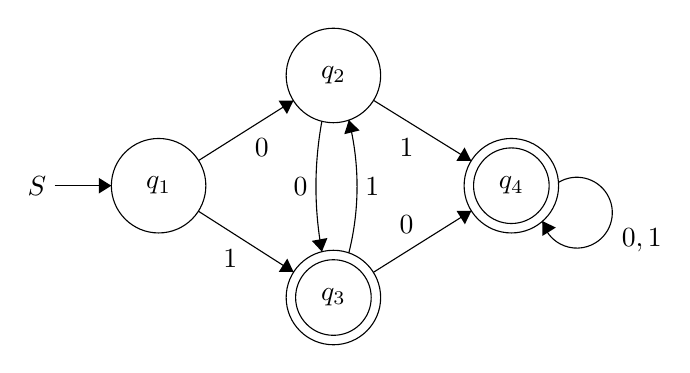
\begin{tikzpicture}[scale=0.2]
		\tikzstyle{every node}+=[inner sep=0pt]
		\draw [black] (22.3,-13.3) circle (3);
		\draw (22.3,-13.3) node {$q_1$};
		\draw [black] (33.4,-6.3) circle (3);
		\draw (33.4,-6.3) node {$q_2$};
		\draw [black] (33.4,-20.4) circle (3);
		\draw (33.4,-20.4) node {$q_3$};
		\draw [black] (33.4,-20.4) circle (2.4);
		\draw [black] (44.7,-13.3) circle (3);
		\draw (44.7,-13.3) node {$q_4$};
		\draw [black] (44.7,-13.3) circle (2.4);
		\draw [black] (24.84,-11.7) -- (30.86,-7.9);
		\fill [black] (30.86,-7.9) -- (29.92,-7.9) -- (30.45,-8.75);
		\draw (28.85,-10.3) node [below] {$0$};
		\draw [black] (24.83,-14.92) -- (30.87,-18.78);
		\fill [black] (30.87,-18.78) -- (30.47,-17.93) -- (29.93,-18.77);
		\draw (26.85,-17.35) node [below] {$1$};
		\draw [black] (35.95,-7.88) -- (42.15,-11.72);
		\fill [black] (42.15,-11.72) -- (41.73,-10.87) -- (41.21,-11.72);
		\draw (38.05,-10.3) node [below] {$1$};
		\draw [black] (35.94,-18.8) -- (42.16,-14.9);
		\fill [black] (42.16,-14.9) -- (41.22,-14.9) -- (41.75,-15.75);
		\draw (38.05,-16.35) node [above] {$0$};
		\draw [black] (32.668,-17.493) arc (-169.60411:-190.39589:22.959);
		\fill [black] (32.67,-17.49) -- (33.02,-16.62) -- (32.03,-16.8);
		\draw (31.79,-13.35) node [left] {$0$};
		\draw [black] (34.38,-9.132) arc (14.11449:-14.11449:17.298);
		\fill [black] (34.38,-9.13) -- (34.09,-10.03) -- (35.06,-9.79);
		\draw (35.4,-13.35) node [right] {$1$};
		\draw [black] (47.681,-13.097) arc (121.61986:-166.38014:2.25);
		\draw (51.68,-16.78) node [right] {$0,1$};
		\fill [black] (46.67,-15.54) -- (46.67,-16.49) -- (47.52,-15.96);
		\draw [black] (15.7,-13.3) -- (19.3,-13.3);
		\draw (15.2,-13.3) node [left] {$S$};
		\fill [black] (19.3,-13.3) -- (18.5,-12.8) -- (18.5,-13.8);
		\end{tikzpicture}
	\end{center}

	\begin{center}
		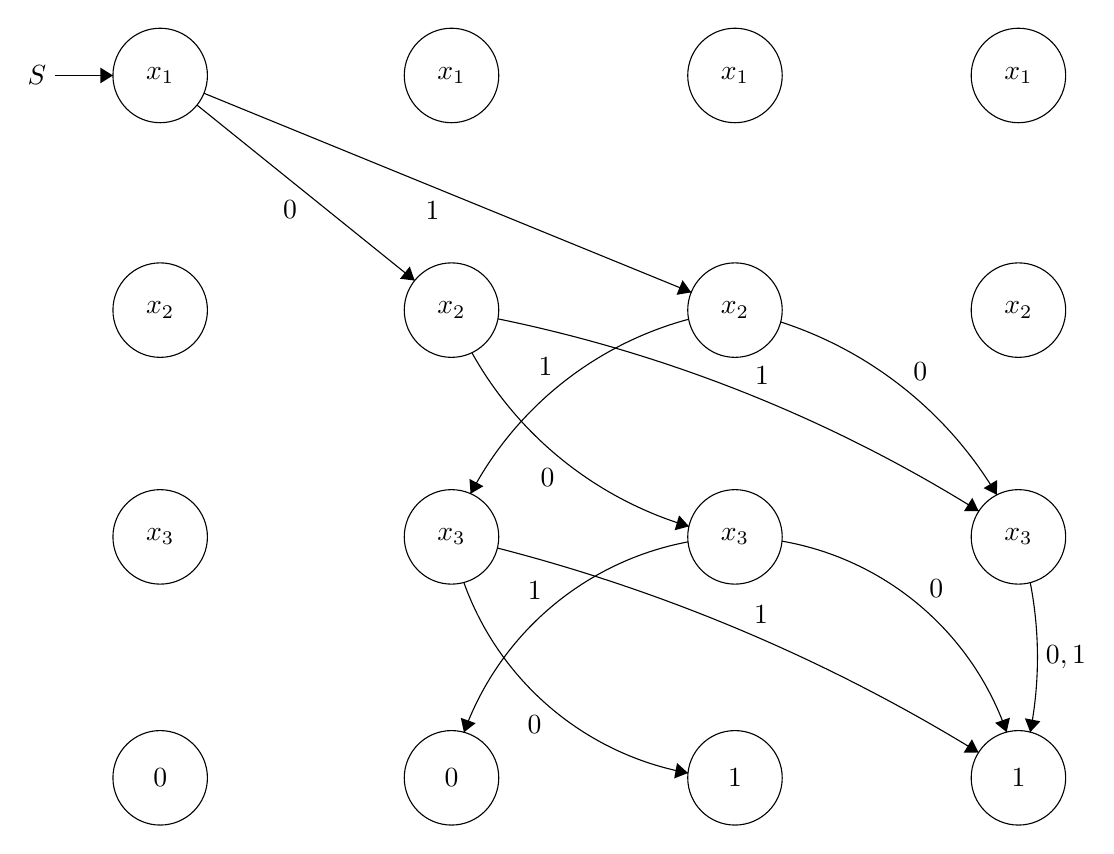
\begin{tikzpicture}[scale=0.2]
		\tikzstyle{every node}+=[inner sep=0pt]
		\draw [black] (11.9,-9) circle (3);
		\draw (11.9,-9) node {$x_1$};
		\draw [black] (30.4,-9) circle (3);
		\draw (30.4,-9) node {$x_1$};
		\draw [black] (48.4,-9) circle (3);
		\draw (48.4,-9) node {$x_1$};
		\draw [black] (66.4,-9) circle (3);
		\draw (66.4,-9) node {$x_1$};
		\draw [black] (11.9,-23.9) circle (3);
		\draw (11.9,-23.9) node {$x_2$};
		\draw [black] (30.4,-23.9) circle (3);
		\draw (30.4,-23.9) node {$x_2$};
		\draw [black] (48.4,-23.9) circle (3);
		\draw (48.4,-23.9) node {$x_2$};
		\draw [black] (66.4,-23.9) circle (3);
		\draw (66.4,-23.9) node {$x_2$};
		\draw [black] (11.9,-38.3) circle (3);
		\draw (11.9,-38.3) node {$x_3$};
		\draw [black] (30.4,-38.3) circle (3);
		\draw (30.4,-38.3) node {$x_3$};
		\draw [black] (48.4,-38.3) circle (3);
		\draw (48.4,-38.3) node {$x_3$};
		\draw [black] (66.4,-38.3) circle (3);
		\draw (66.4,-38.3) node {$x_3$};
		\draw [black] (11.9,-53.6) circle (3);
		\draw (11.9,-53.6) node {$0$};
		\draw [black] (30.4,-53.6) circle (3);
		\draw (30.4,-53.6) node {$0$};
		\draw [black] (48.4,-53.6) circle (3);
		\draw (48.4,-53.6) node {$1$};
		\draw [black] (66.4,-53.6) circle (3);
		\draw (66.4,-53.6) node {$1$};
		\draw [black] (5.2,-9) -- (8.9,-9);
		\draw (4.7,-9) node [left] {$S$};
		\fill [black] (8.9,-9) -- (8.1,-8.5) -- (8.1,-9.5);
		\draw [black] (14.24,-10.88) -- (28.06,-22.02);
		\fill [black] (28.06,-22.02) -- (27.75,-21.13) -- (27.13,-21.91);
		\draw (20.14,-16.94) node [below] {$0$};
		\draw [black] (14.68,-10.13) -- (45.62,-22.77);
		\fill [black] (45.62,-22.77) -- (45.07,-22) -- (44.69,-22.93);
		\draw (29.19,-16.97) node [below] {$1$};
		\draw [black] (33.348,-24.455) arc (78.40934:57.98784:92.758);
		\fill [black] (63.88,-36.67) -- (63.47,-35.82) -- (62.94,-36.67);
		\draw (50.12,-28.68) node [above] {$1$};
		\draw [black] (45.477,-37.632) arc (-106.53781:-150.78181:23.438);
		\fill [black] (45.48,-37.63) -- (44.85,-36.93) -- (44.57,-37.88);
		\draw (36.5,-33.96) node [below] {$0$};
		\draw [black] (51.302,-24.652) arc (72.0185:30.66188:24.891);
		\fill [black] (65.03,-35.63) -- (65.05,-34.69) -- (64.19,-35.2);
		\draw (60.17,-28.4) node [above] {$0$};
		\draw [black] (31.611,-35.558) arc (152.28216:105.03745:22.128);
		\fill [black] (31.61,-35.56) -- (32.43,-35.08) -- (31.54,-34.62);
		\draw (36.37,-28.08) node [above] {$1$};
		\draw [black] (45.419,-53.295) arc (-100.43541:-160.29366:18.726);
		\fill [black] (45.42,-53.29) -- (44.72,-52.66) -- (44.54,-53.64);
		\draw (35.67,-49.64) node [below] {$0$};
		\draw [black] (33.315,-39.008) arc (75.57252:58.3765:111.025);
		\fill [black] (63.87,-51.99) -- (63.45,-51.15) -- (62.92,-52);
		\draw (50.05,-43.84) node [above] {$1$};
		\draw [black] (51.384,-38.571) arc (80.14942:19.12151:18.439);
		\fill [black] (65.65,-50.7) -- (65.86,-49.78) -- (64.92,-50.11);
		\draw (61.18,-42.2) node [above] {$0$};
		\draw [black] (31.192,-50.71) arc (160.10675:100.62232:18.82);
		\fill [black] (31.19,-50.71) -- (31.93,-50.13) -- (30.99,-49.79);
		\draw (35.69,-42.28) node [above] {$1$};
		\draw [black] (67.15,-41.203) arc (11.02807:-11.02807:24.817);
		\fill [black] (67.15,-50.7) -- (67.79,-50.01) -- (66.81,-49.82);
		\draw (68.11,-45.95) node [right] {$0,1$};
		\end{tikzpicture}
	\end{center}

	%       10.19       %
	\item[10.19]
	Obviously RP $ \subseteq $ NP. We only need to show that if NP $ \subseteq $ BPP then NP $ \subseteq $ RP. Since SAT is NP complete, we only need to show SAT $ \in $ RP. Given a formula $ \phi $ with $ m $ variables, find a BPP algorithm B with error probability $ 2^{-m-1} $ (the assumption that SAT $ \in $ BPP guarantees this). We can run B on $ \phi $, if it rejects then the RP algorithm R rejects. Otherwise we randomly choose an assignment to the variable $ x_1 $ and run B on the reduced formula. If it rejects then we change the value of $ x_1 $. Then we perform similar steps for $ x_2 $, $ x_3 $, ..., $ x_m $, and in the end test whether the resulting formula is true and we accept or reject accordingly.
	
	%       10.20       %
	\item[10.20]
	See \url{https://en.wikipedia.org/wiki/ZPP_(complexity)#Intersection_definition}
	
	One note for tackling the difference between worst-time and averaged-time: take the time consumed on a random input as a random variable, and apply Markov's Inequality to it.
	
	%       10.21       %
	\item[10.21]
	Show that $ 3SAT \le_P \overline{EQ_{BP}} $: $ \phi \in 3SAT $ iff $ L(B1) \ne L(B2) $, where $ B_1 $ is a branching program which unconditionally outputs 0 and $ B_2 $ is a branching program constructed from $ \phi $ so that $ \phi $ is satisfiable iff $ B_2 $ can reach the output node 1 with the corresponding assignment of variables.
	
	%       10.22       %
	\item[10.22]
	Suppose A is a language that is decided by a probabilistic logarithmic space
	TM M with error probability $ \frac{1}{3} $, we can construct a polynomial time algorithm that calculates the probability that string $ w $ of length $ n $ is accepted by M. Then we compare it with $ \frac{2}{3} $. The algorithm is described as follows.
	
	First, build a graph G according to M and $ w $. The vertices of G are possible configurations of M under input string $ w $ (see \textit{Definition 8.20} for the definition of configuration under current context) and the directed edges of G show whether a configuration can be transited into another within one deterministic step or one flip-coin step of M.
	
	We claim that G is a DAG, because otherwise M is not a decider for string $ w $ (it can fall into loops and never terminate). Also, since M runs in logarithmic space, the size of G is bounded by some polynomial of $ n $.
	
	Then, we can calculate the acceptance probability on G in polynomial time using techniques of topological sorting and dynamic programming.
	
\end{itemize}

	
\end{document}